\section*{Question 8}
\fakesection{8}

This exercise extends Question 7 to investigate how stability is impacted by increasing the order of the Butterworth filter. The following filter orders are investigated: 5, 6, 7, and 8.

We begin with the 5th-order low pass Butterworth filter.

\begin{figure}[ht]
    \centering
    \begin{subfigure}[b]{0.58\textwidth}
        \centering
        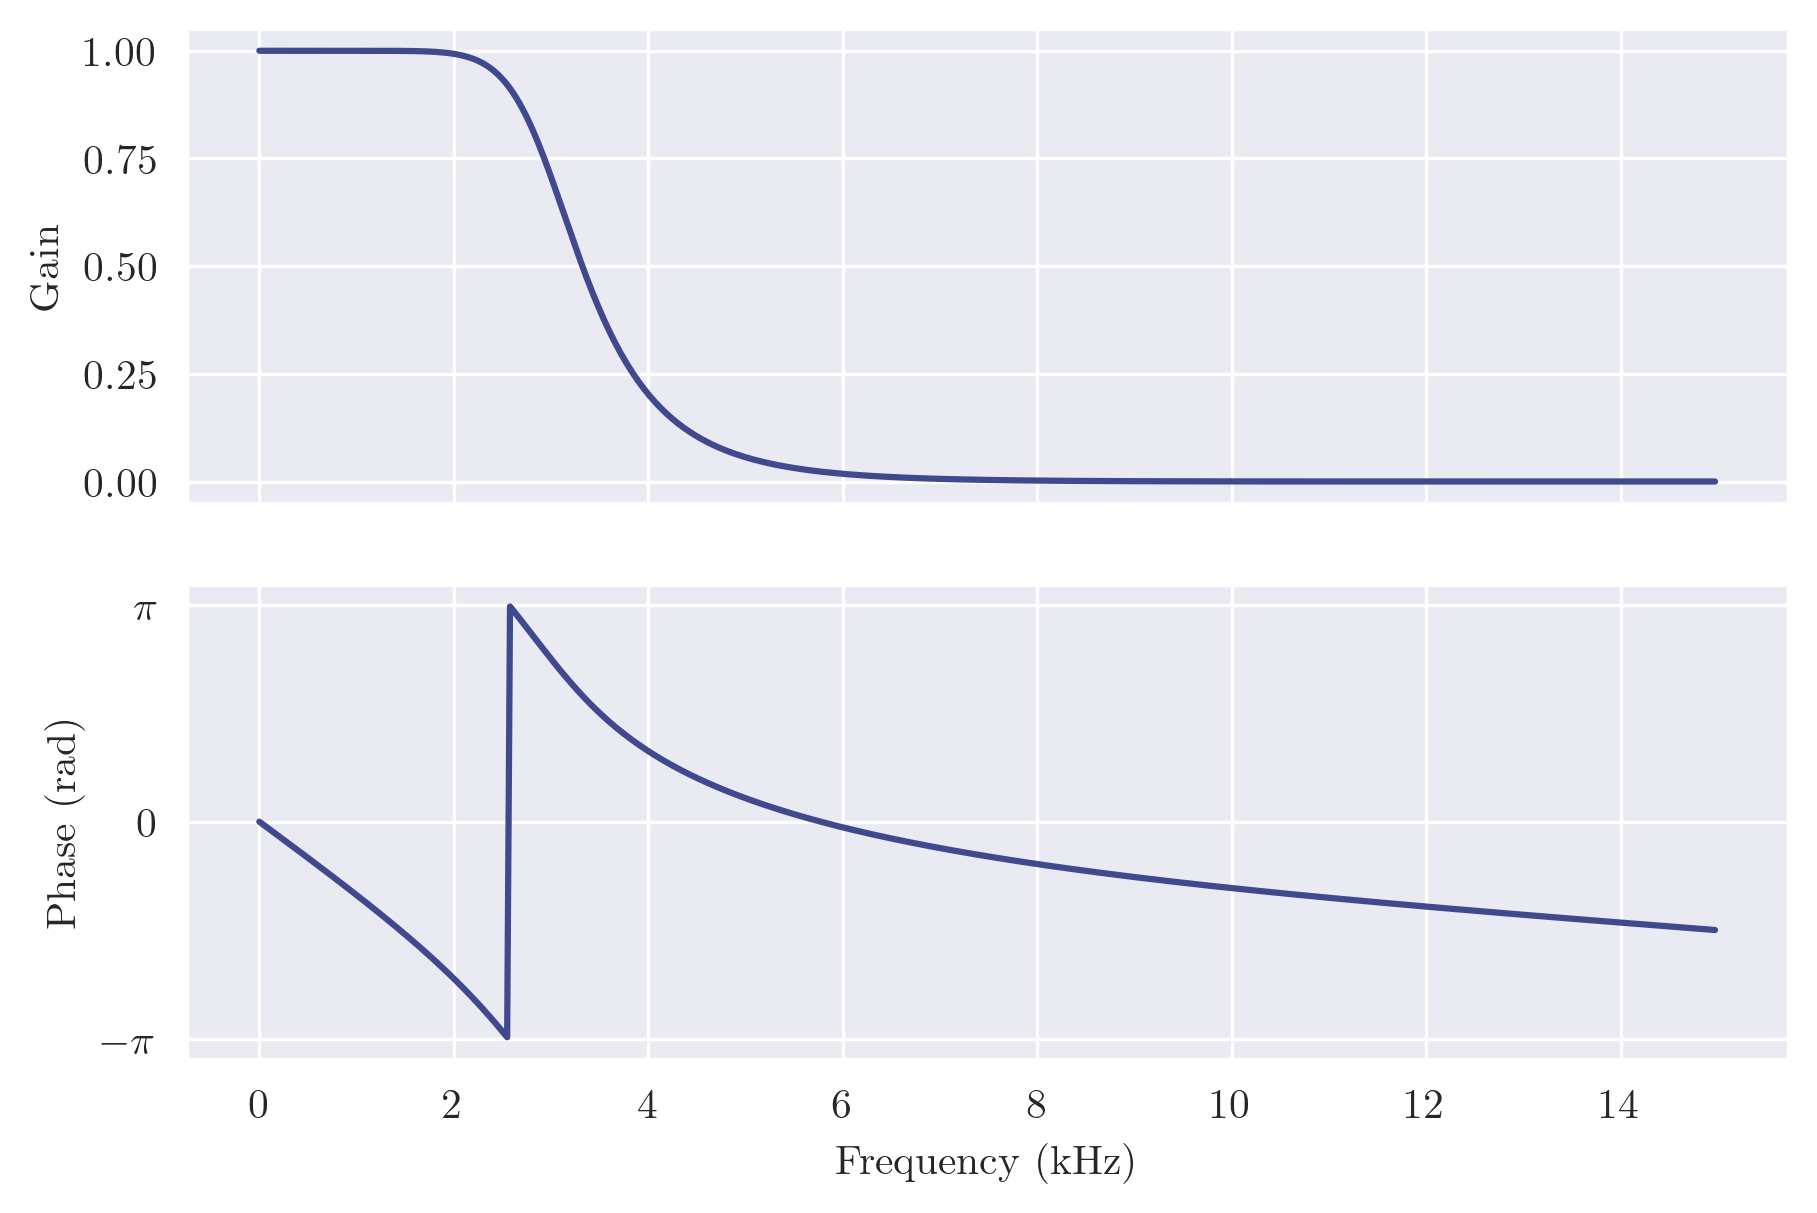
\includegraphics[width=\textwidth]{images/q8_5th_freqz.png}
    \end{subfigure}
    \hfill
    \begin{subfigure}[b]{0.41\textwidth}
        \centering
        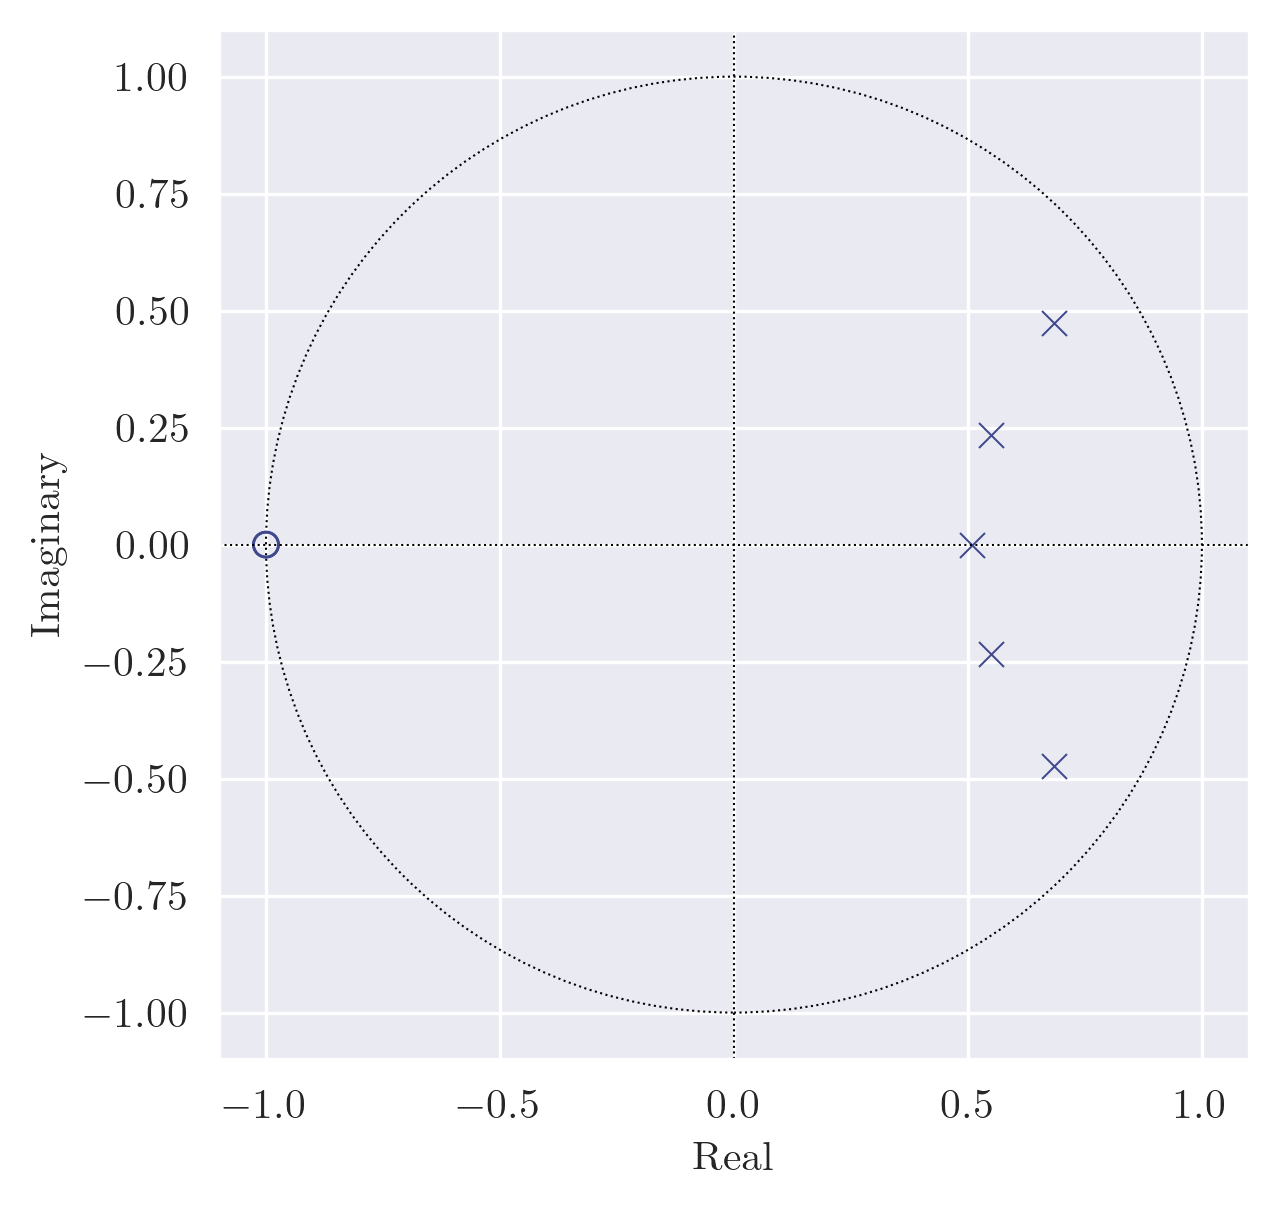
\includegraphics[width=\textwidth]{images/q8_5th_zp.png}
    \end{subfigure}
    \caption{Frequency response and pole-zero plot of 5th-order low pass Butterworth filter}
\end{figure}

We then quantize the filter coefficients and repeat, observing changes in the pole-zero plot.

\begin{figure}[!ht]
    \centering
    \begin{subfigure}[b]{0.58\textwidth}
        \centering
        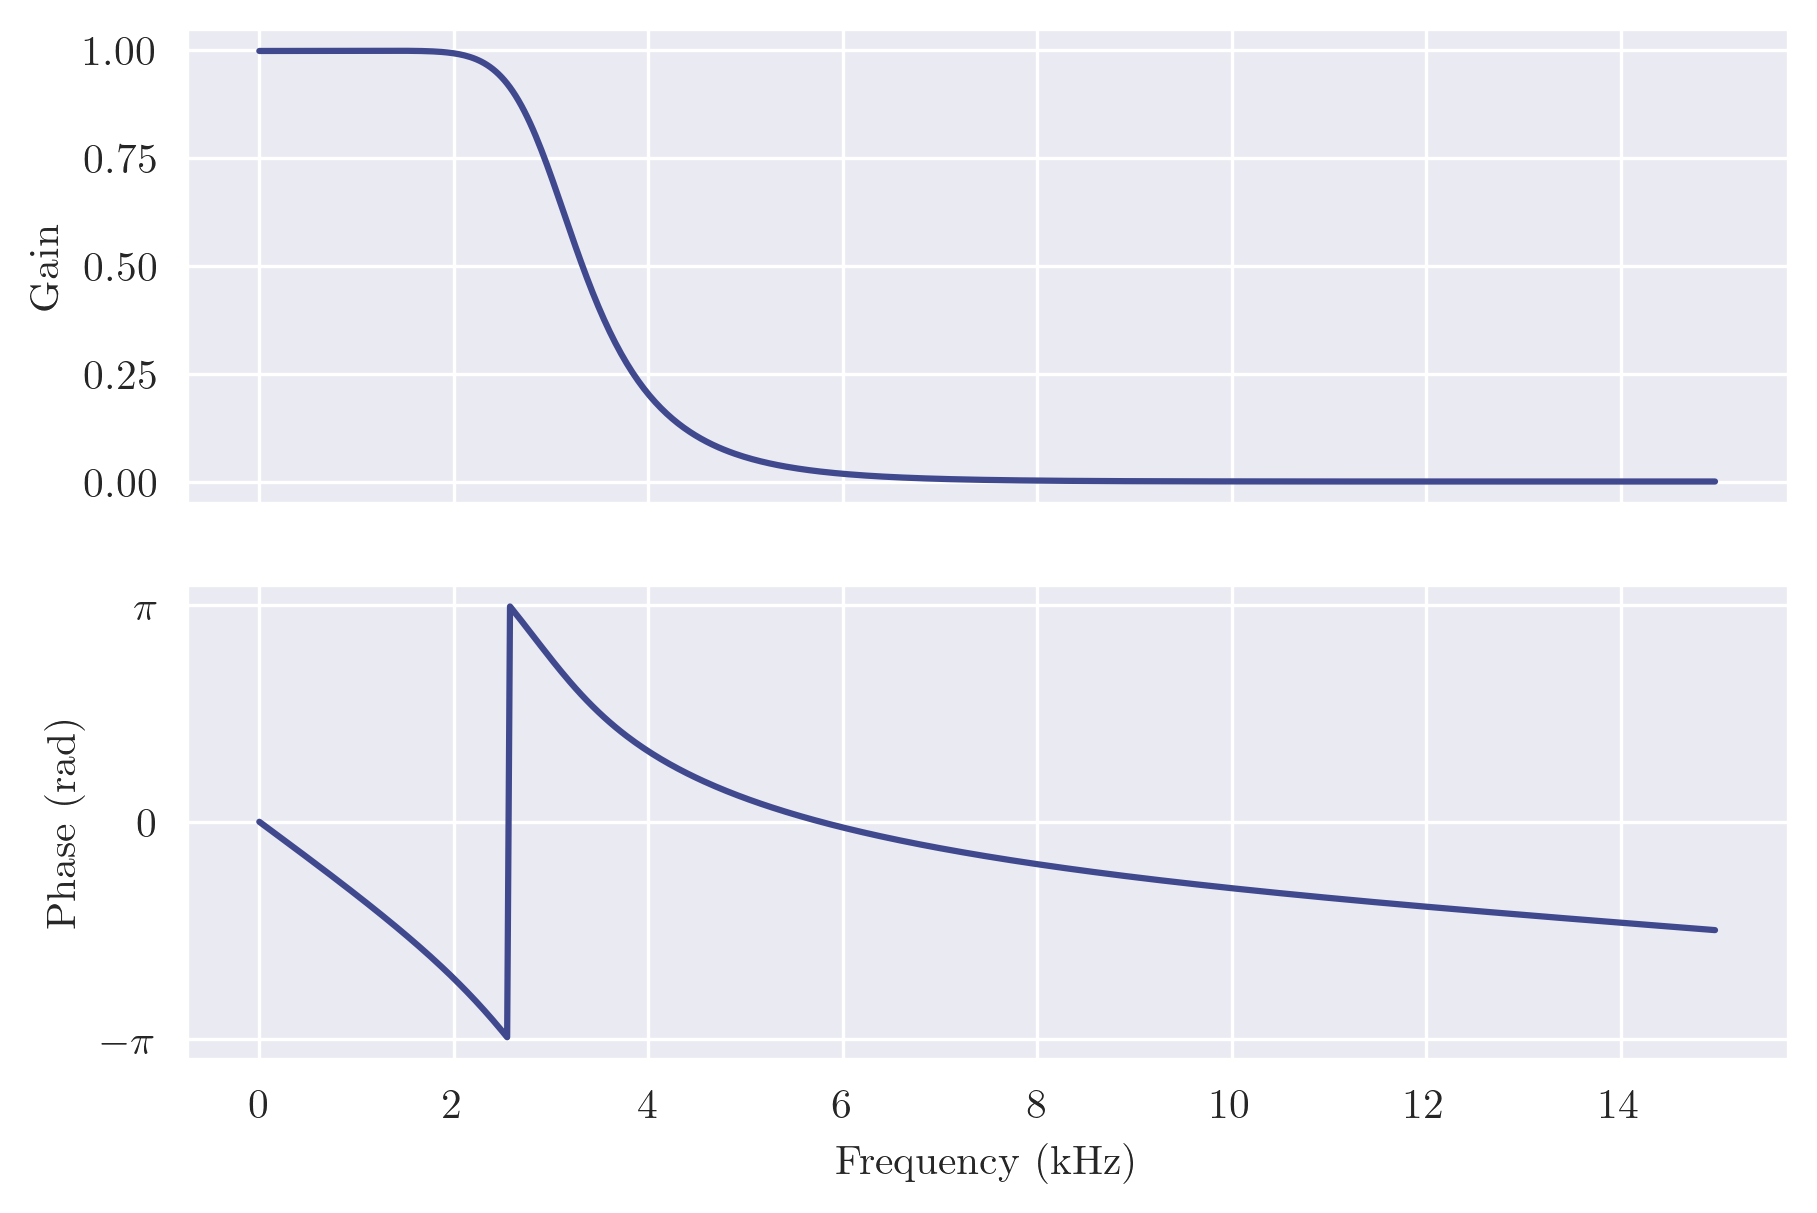
\includegraphics[width=\textwidth]{images/q8_q5th_freqz.png}
    \end{subfigure}
    \hfill
    \begin{subfigure}[b]{0.41\textwidth}
        \centering
        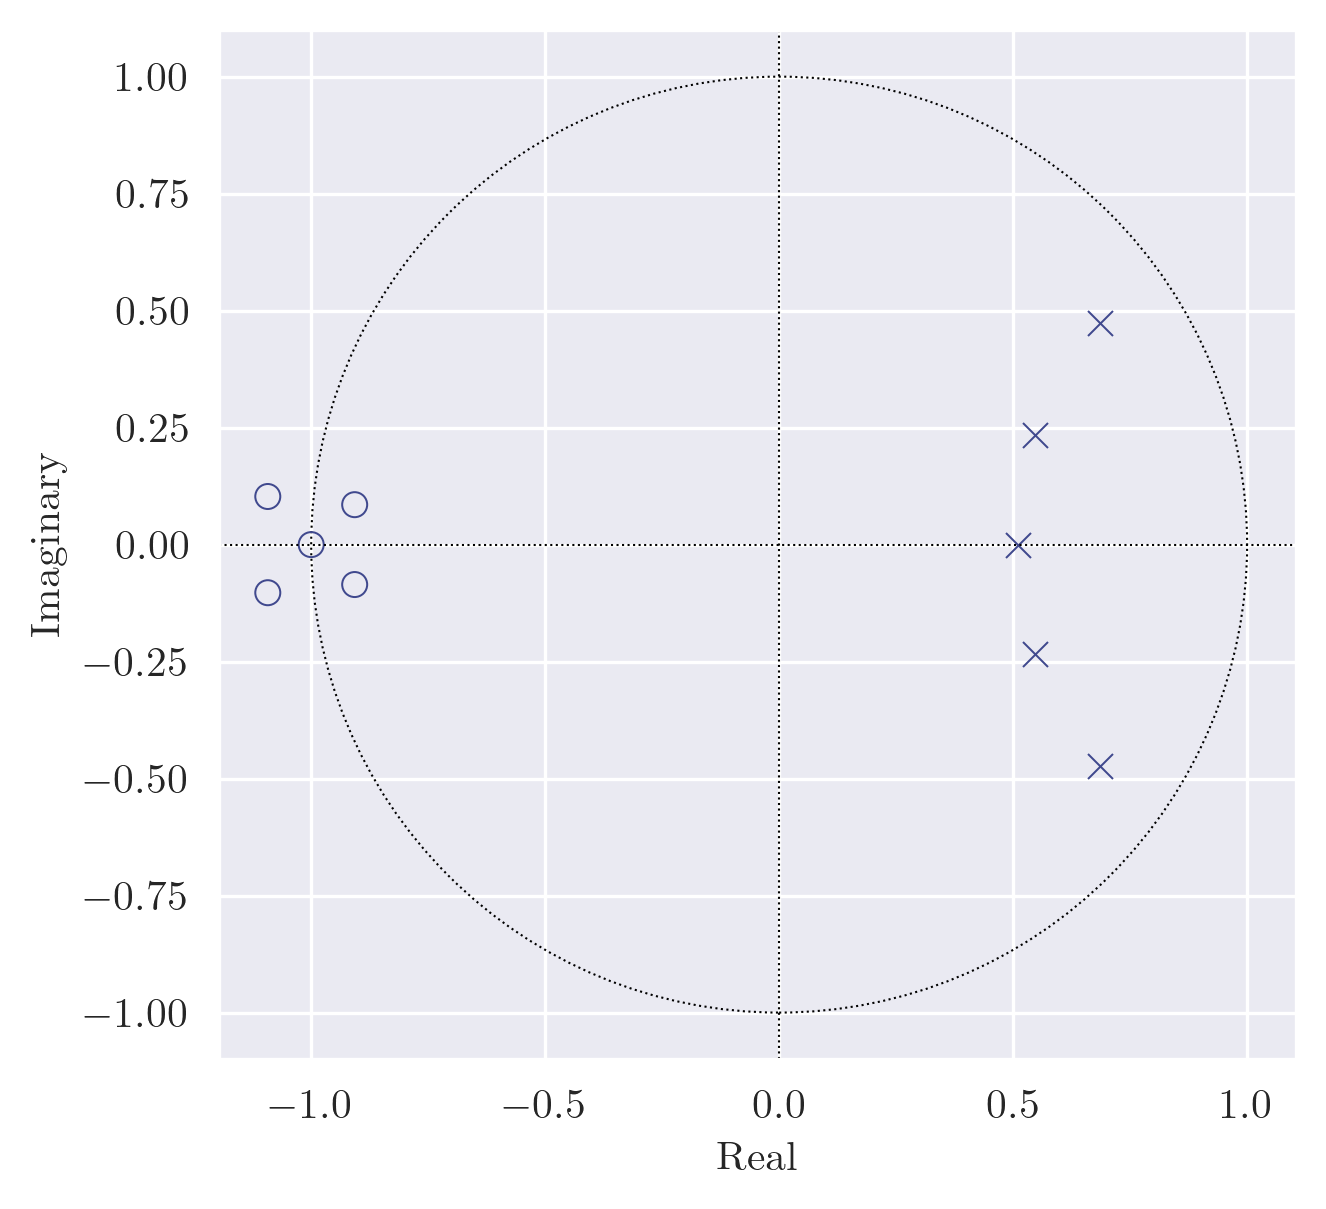
\includegraphics[width=\textwidth]{images/q8_q5th_zp.png}
    \end{subfigure}
    \caption{Frequency response and pole-zero plot of quantized 5th-order filter}
\end{figure}

\textit{TODO: describe observed differences}

\newpage

We now attempt a 6th-order low pass Butterworth filter.

\begin{figure}[ht]
    \centering
    \begin{subfigure}[b]{0.58\textwidth}
        \centering
        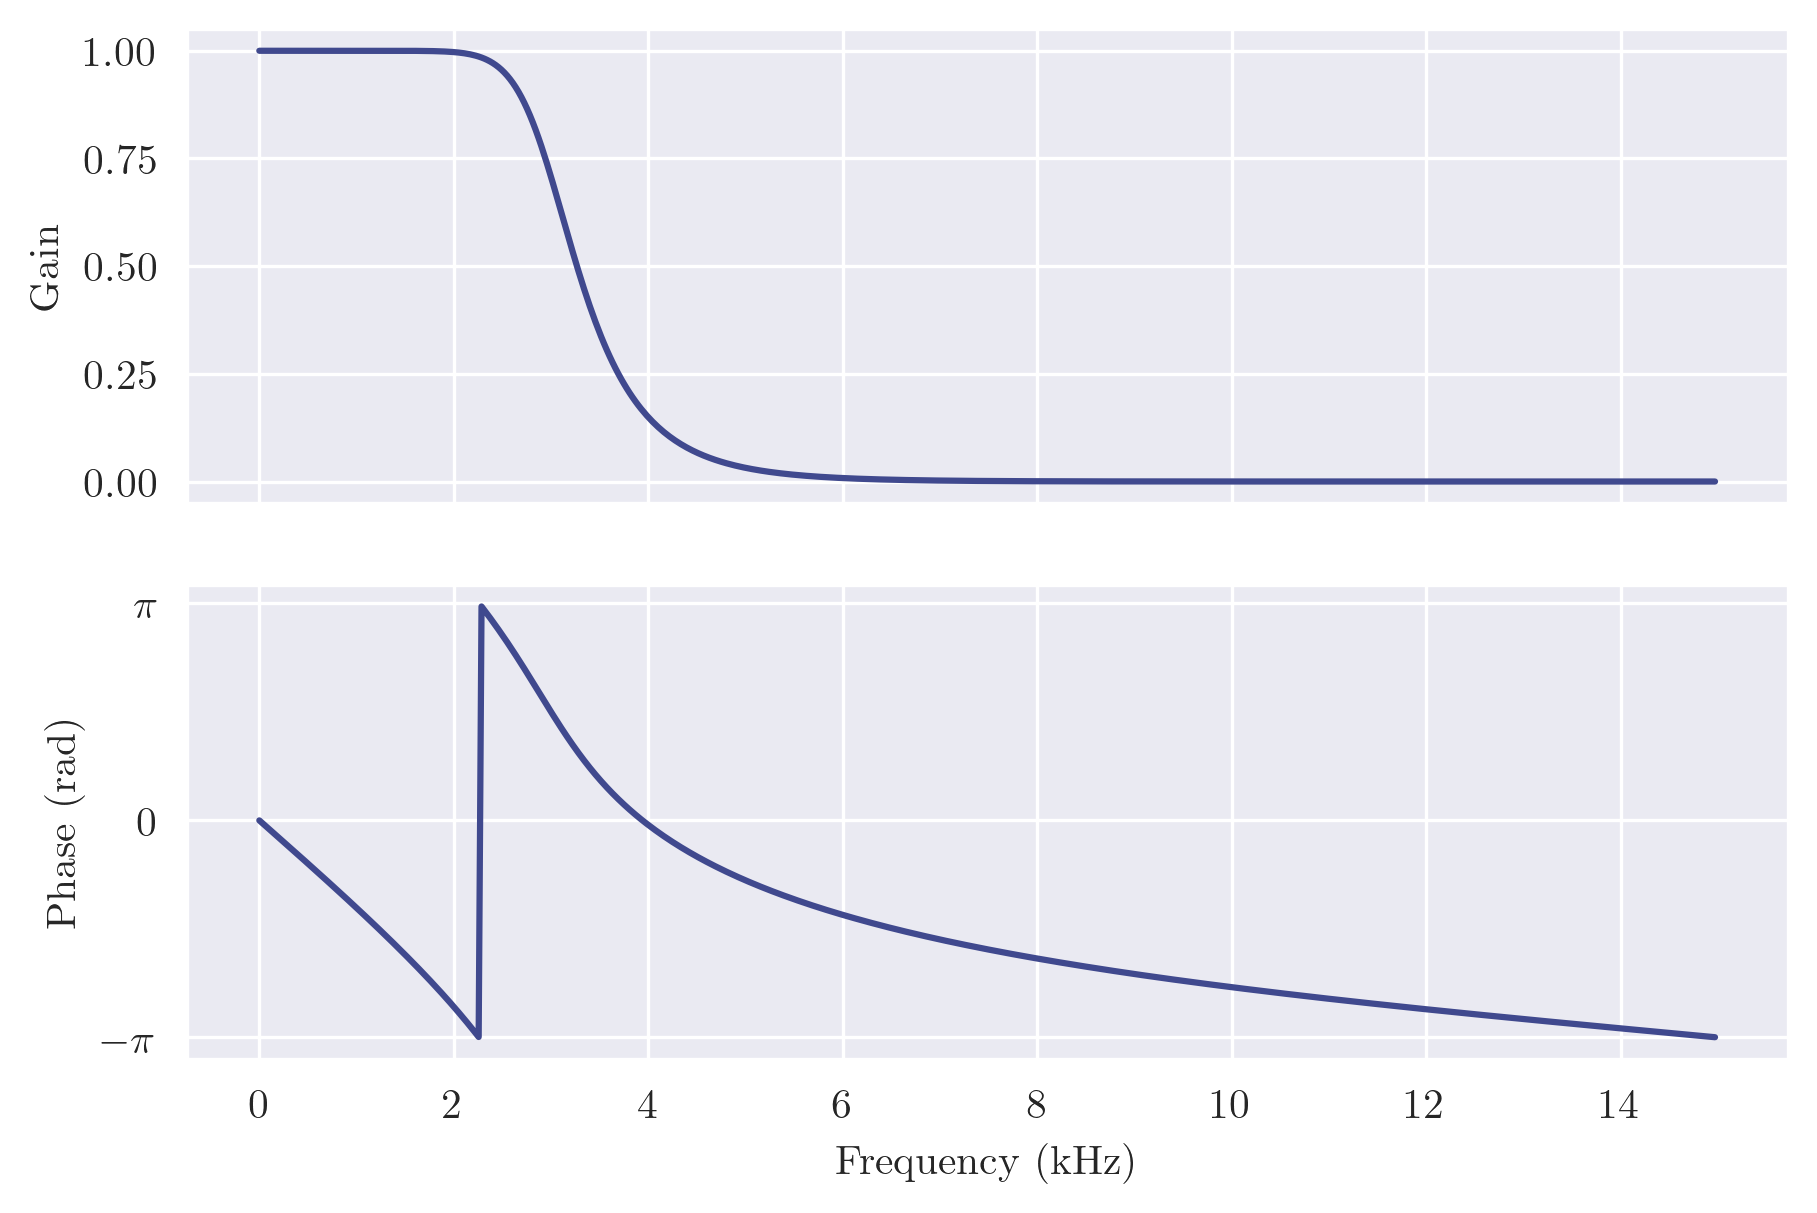
\includegraphics[width=\textwidth]{images/q8_6th_freqz.png}
    \end{subfigure}
    \hfill
    \begin{subfigure}[b]{0.41\textwidth}
        \centering
        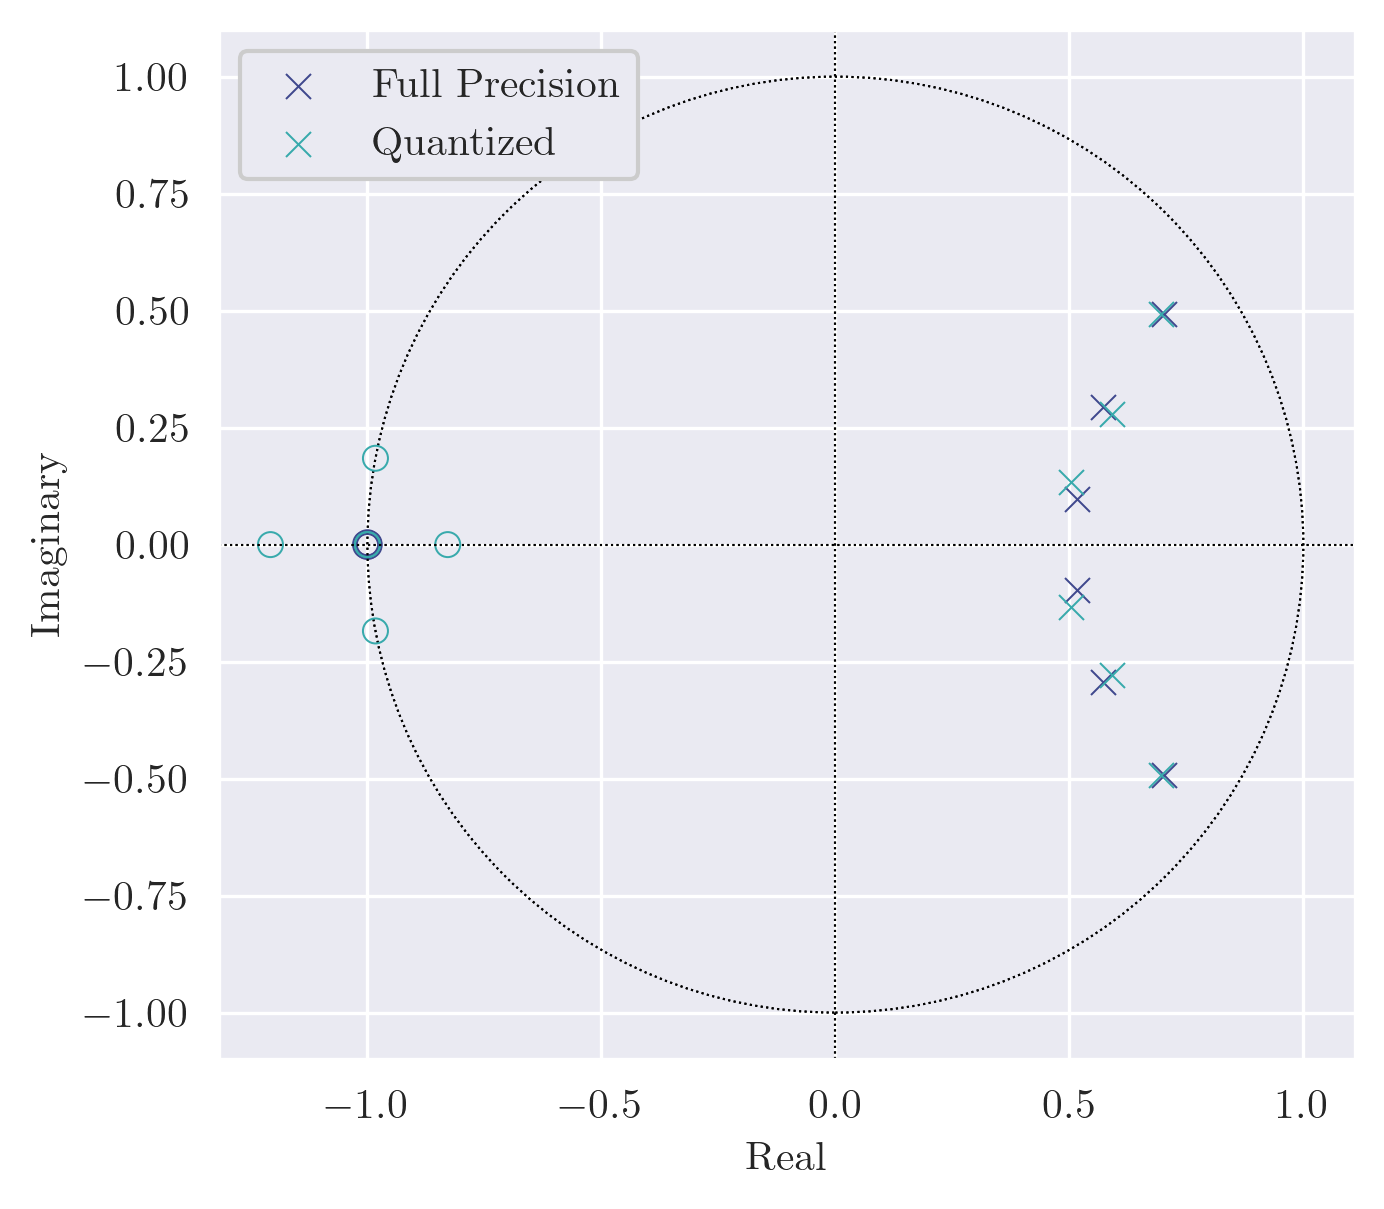
\includegraphics[width=\textwidth]{images/q8_6th_zp.png}
    \end{subfigure}
    \caption{Frequency response and pole-zero plot of 6th-order low pass Butterworth filter}
\end{figure}

We then quantize the filter coefficients and repeat, observing changes in the pole-zero plot.

\begin{figure}[!ht]
    \centering
    \begin{subfigure}[b]{0.58\textwidth}
        \centering
        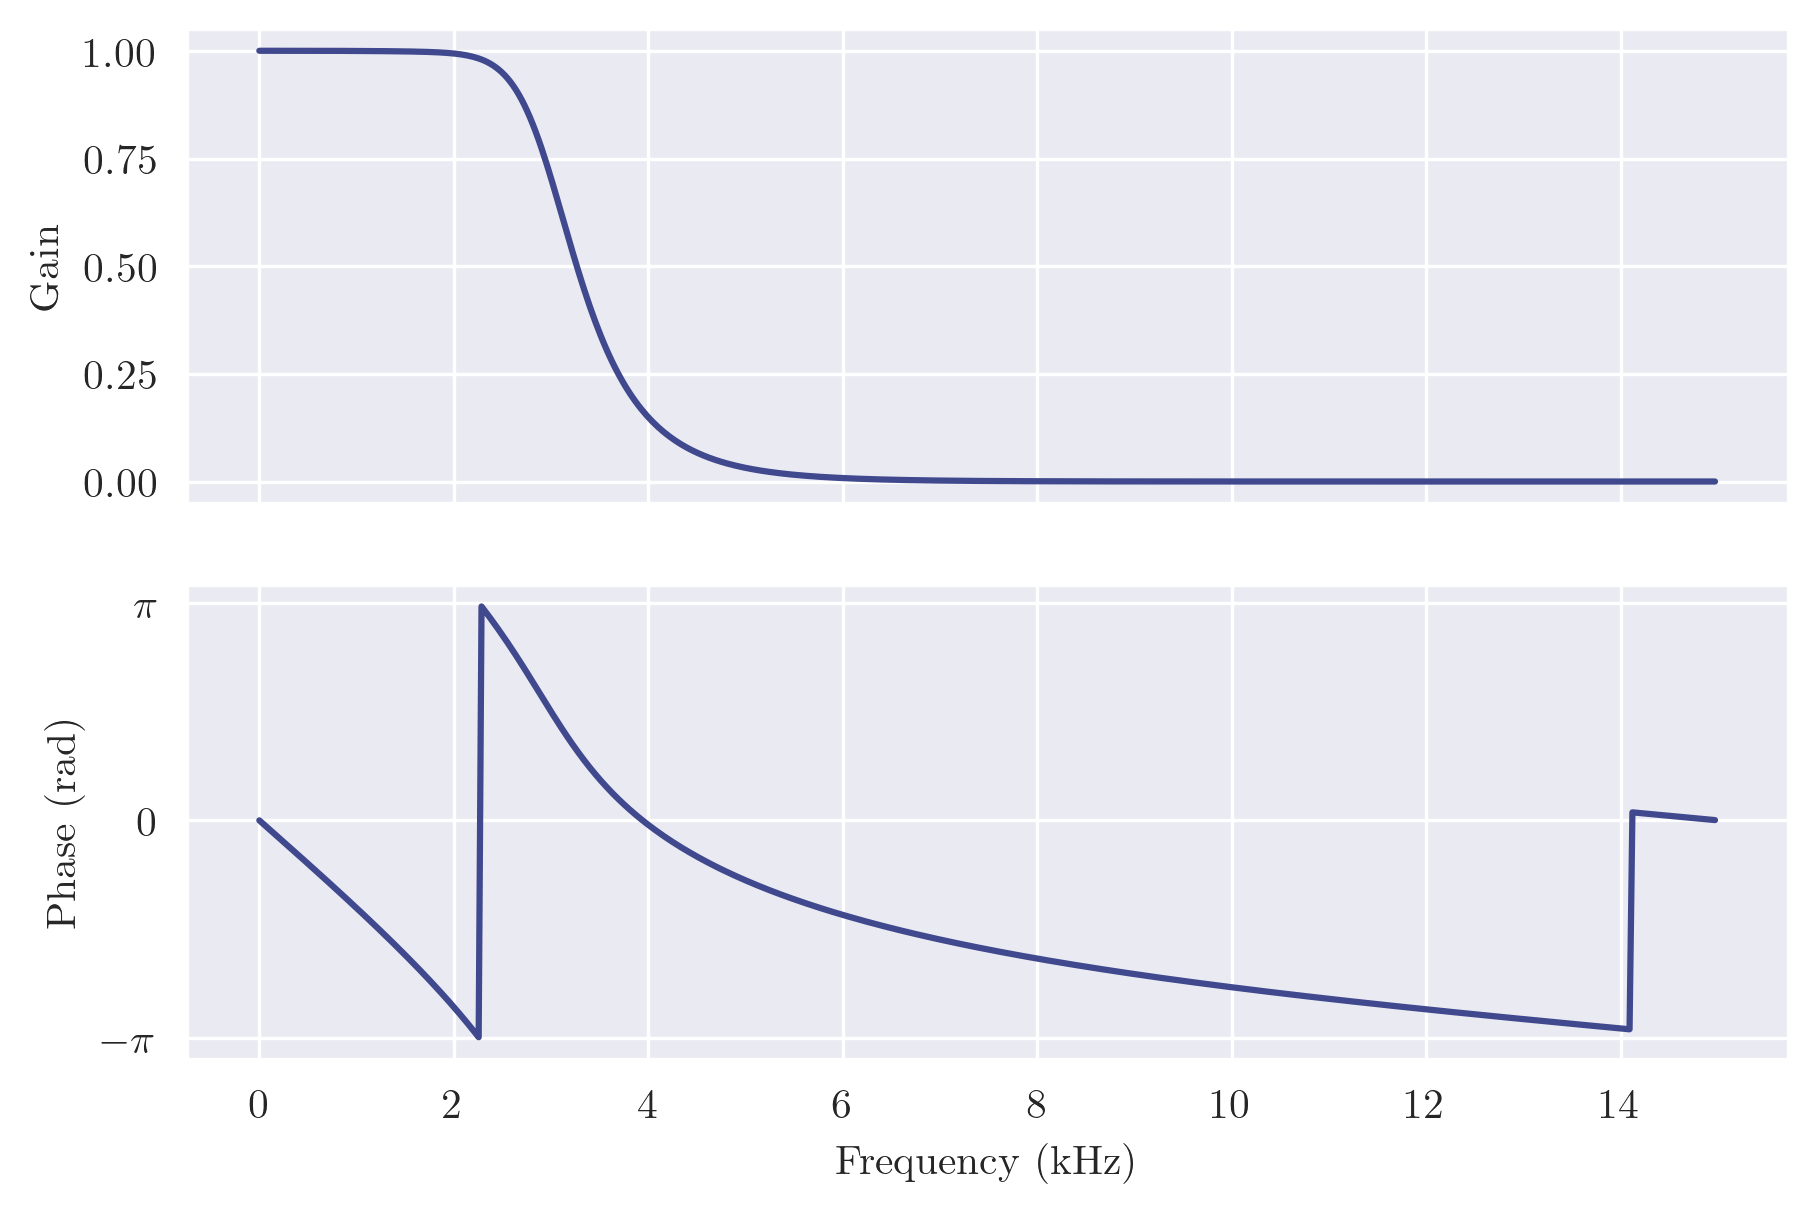
\includegraphics[width=\textwidth]{images/q8_q6th_freqz.png}
    \end{subfigure}
    \hfill
    \begin{subfigure}[b]{0.41\textwidth}
        \centering
        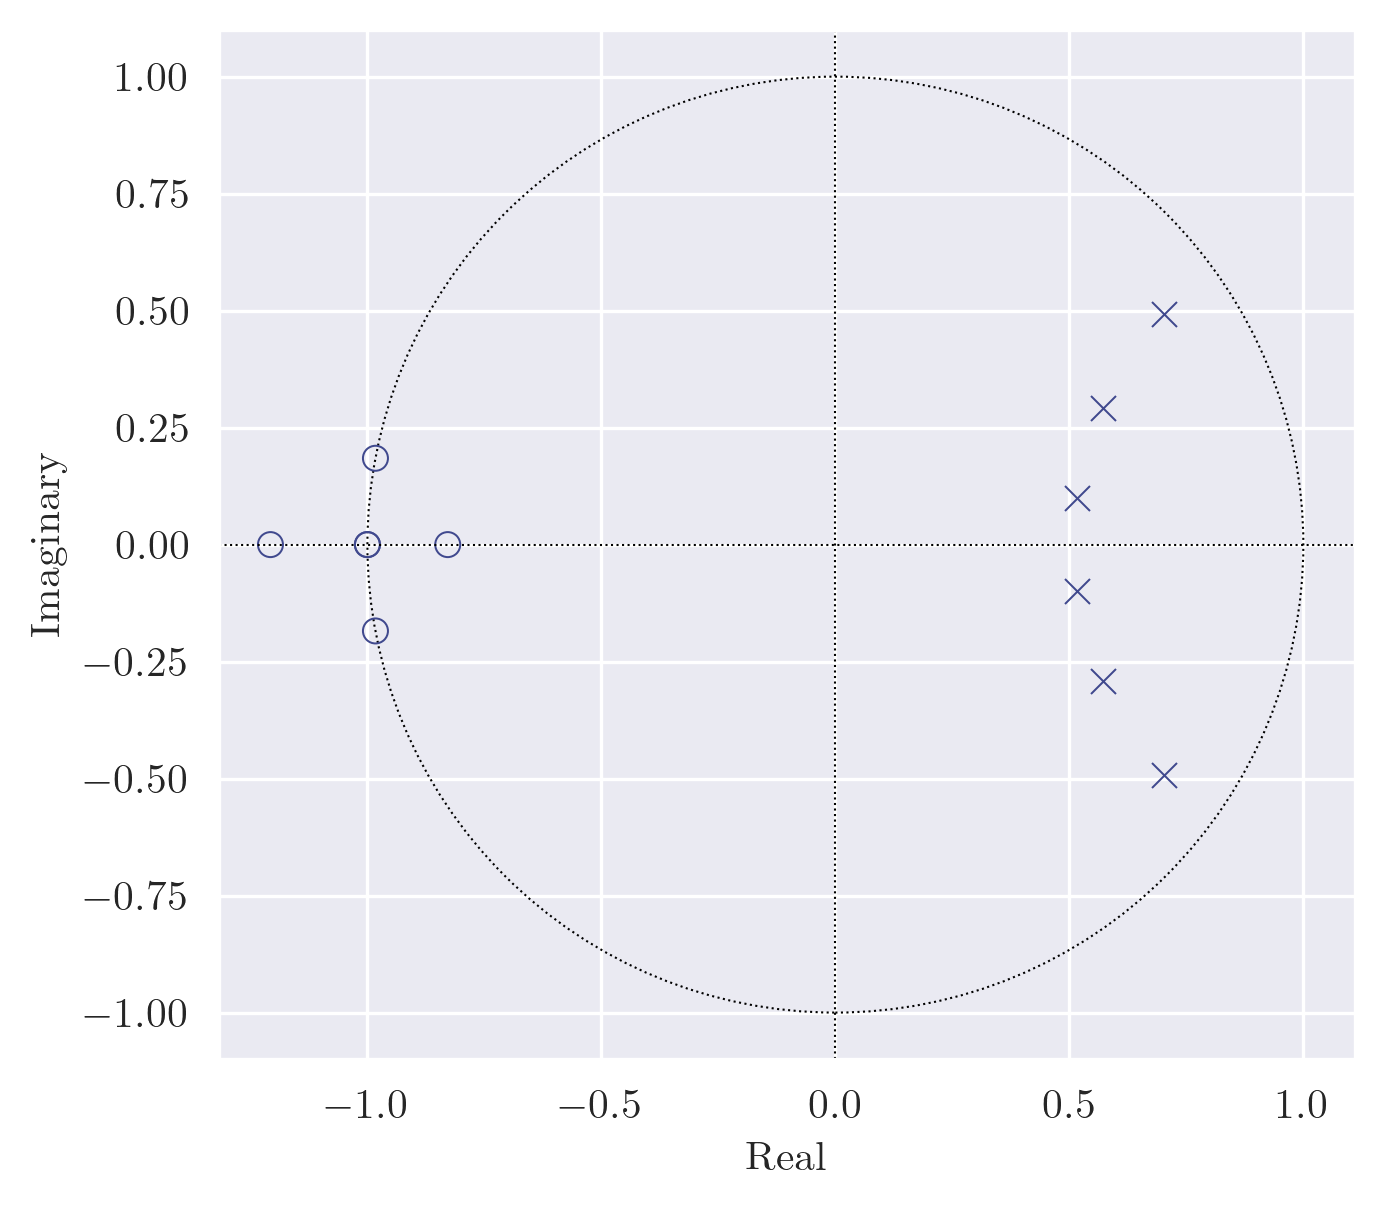
\includegraphics[width=\textwidth]{images/q8_q6th_zp.png}
    \end{subfigure}
    \caption{Frequency response and pole-zero plot of quantized 6th-order filter}
\end{figure}

\textit{TODO: describe observed differences}

\newpage

We now attempt a 7th-order low pass Butterworth filter.

\begin{figure}[ht]
    \centering
    \begin{subfigure}[b]{0.58\textwidth}
        \centering
        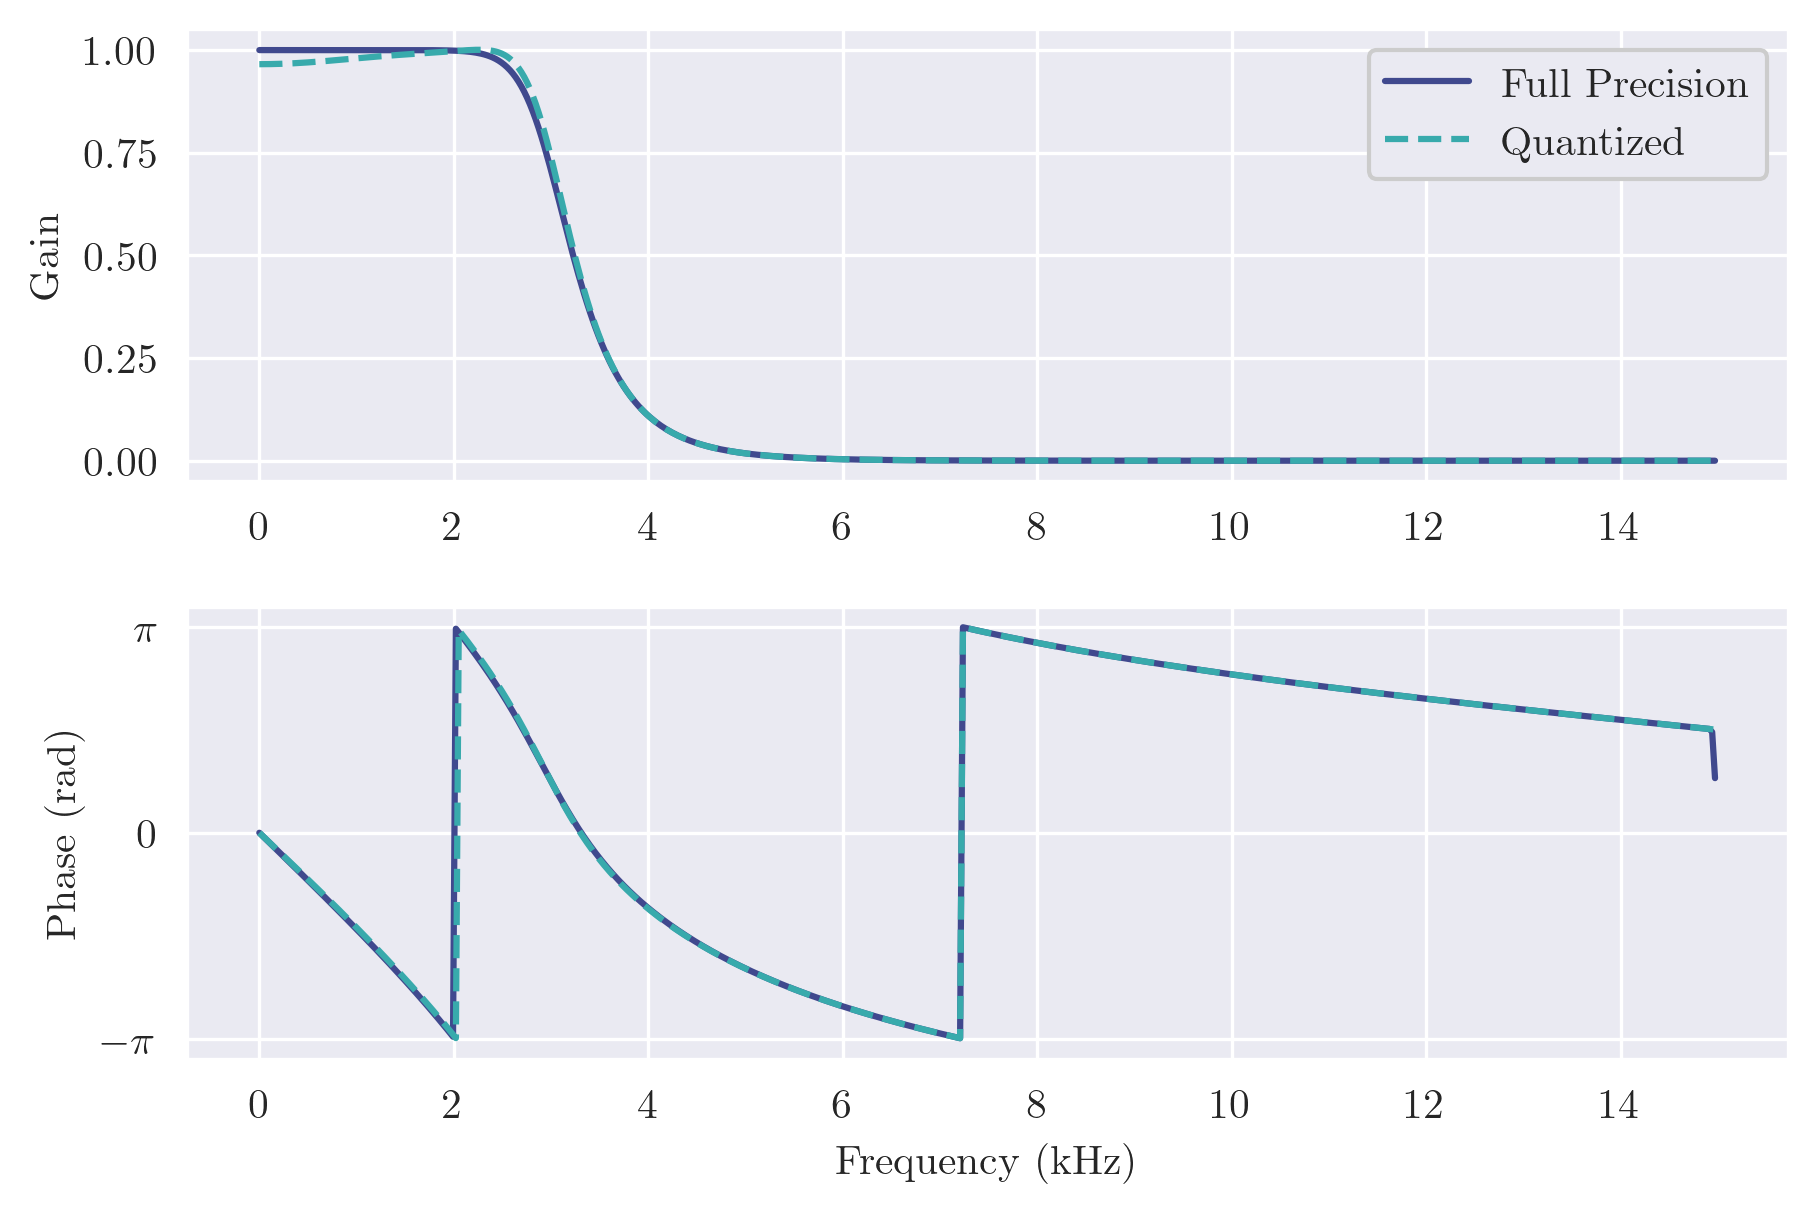
\includegraphics[width=\textwidth]{images/q8_7th_freqz.png}
    \end{subfigure}
    \hfill
    \begin{subfigure}[b]{0.41\textwidth}
        \centering
        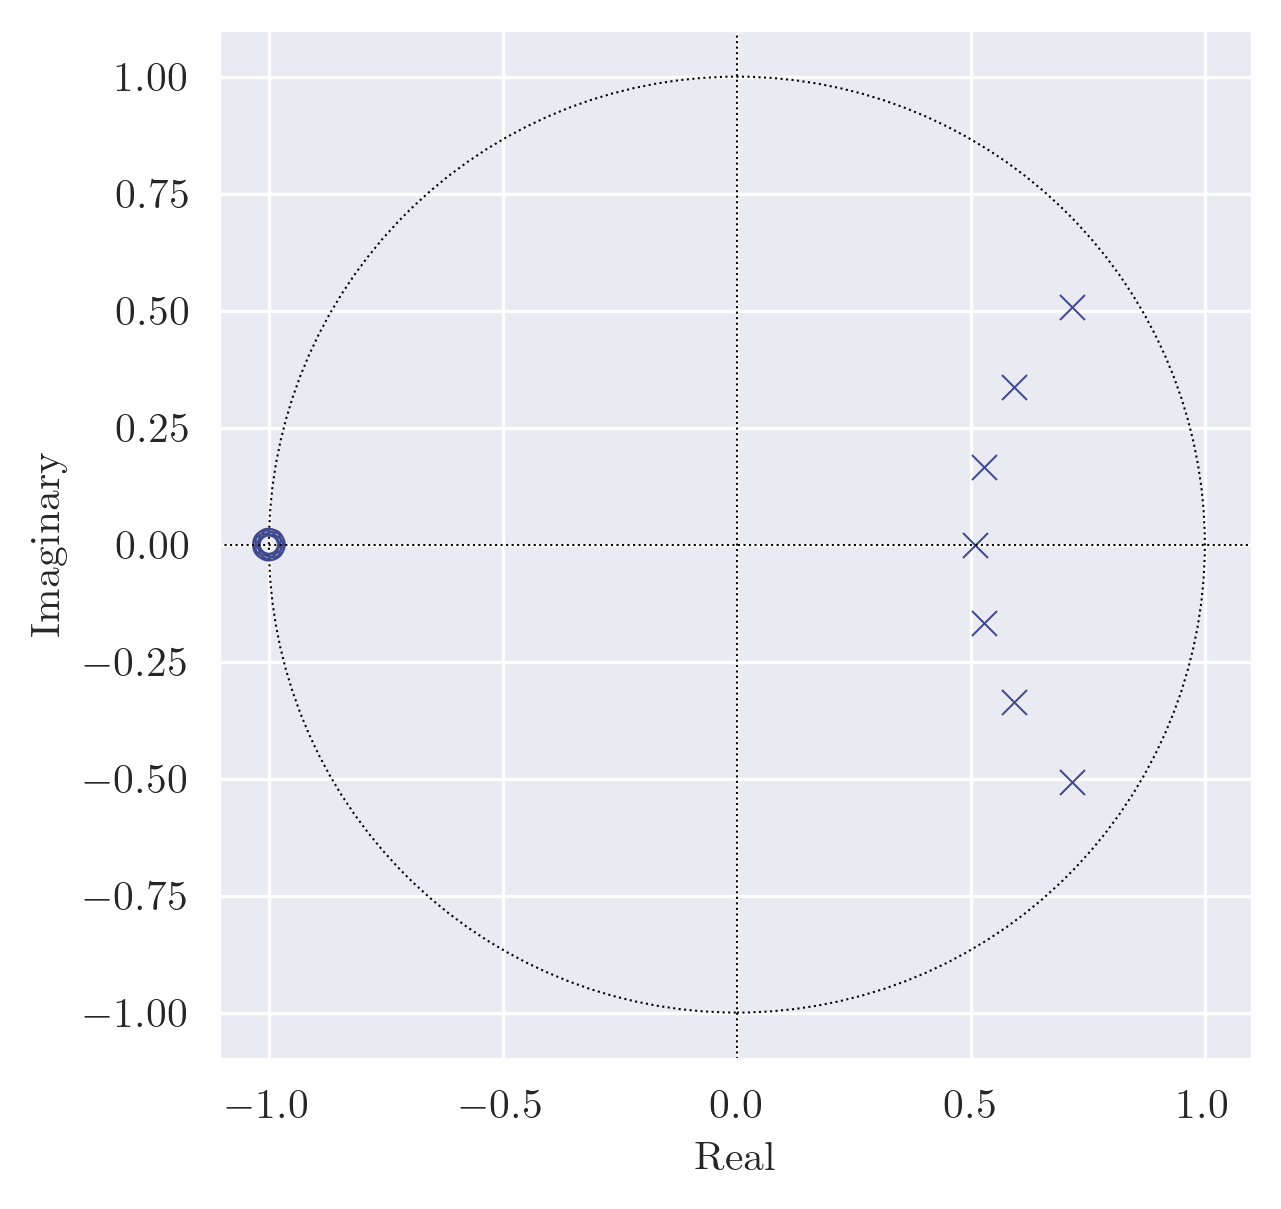
\includegraphics[width=\textwidth]{images/q8_7th_zp.png}
    \end{subfigure}
    \caption{Frequency response and pole-zero plot of 7th-order low pass Butterworth filter}
\end{figure}

We then quantize the filter coefficients and repeat, observing changes in the pole-zero plot.

\begin{figure}[!ht]
    \centering
    \begin{subfigure}[b]{0.58\textwidth}
        \centering
        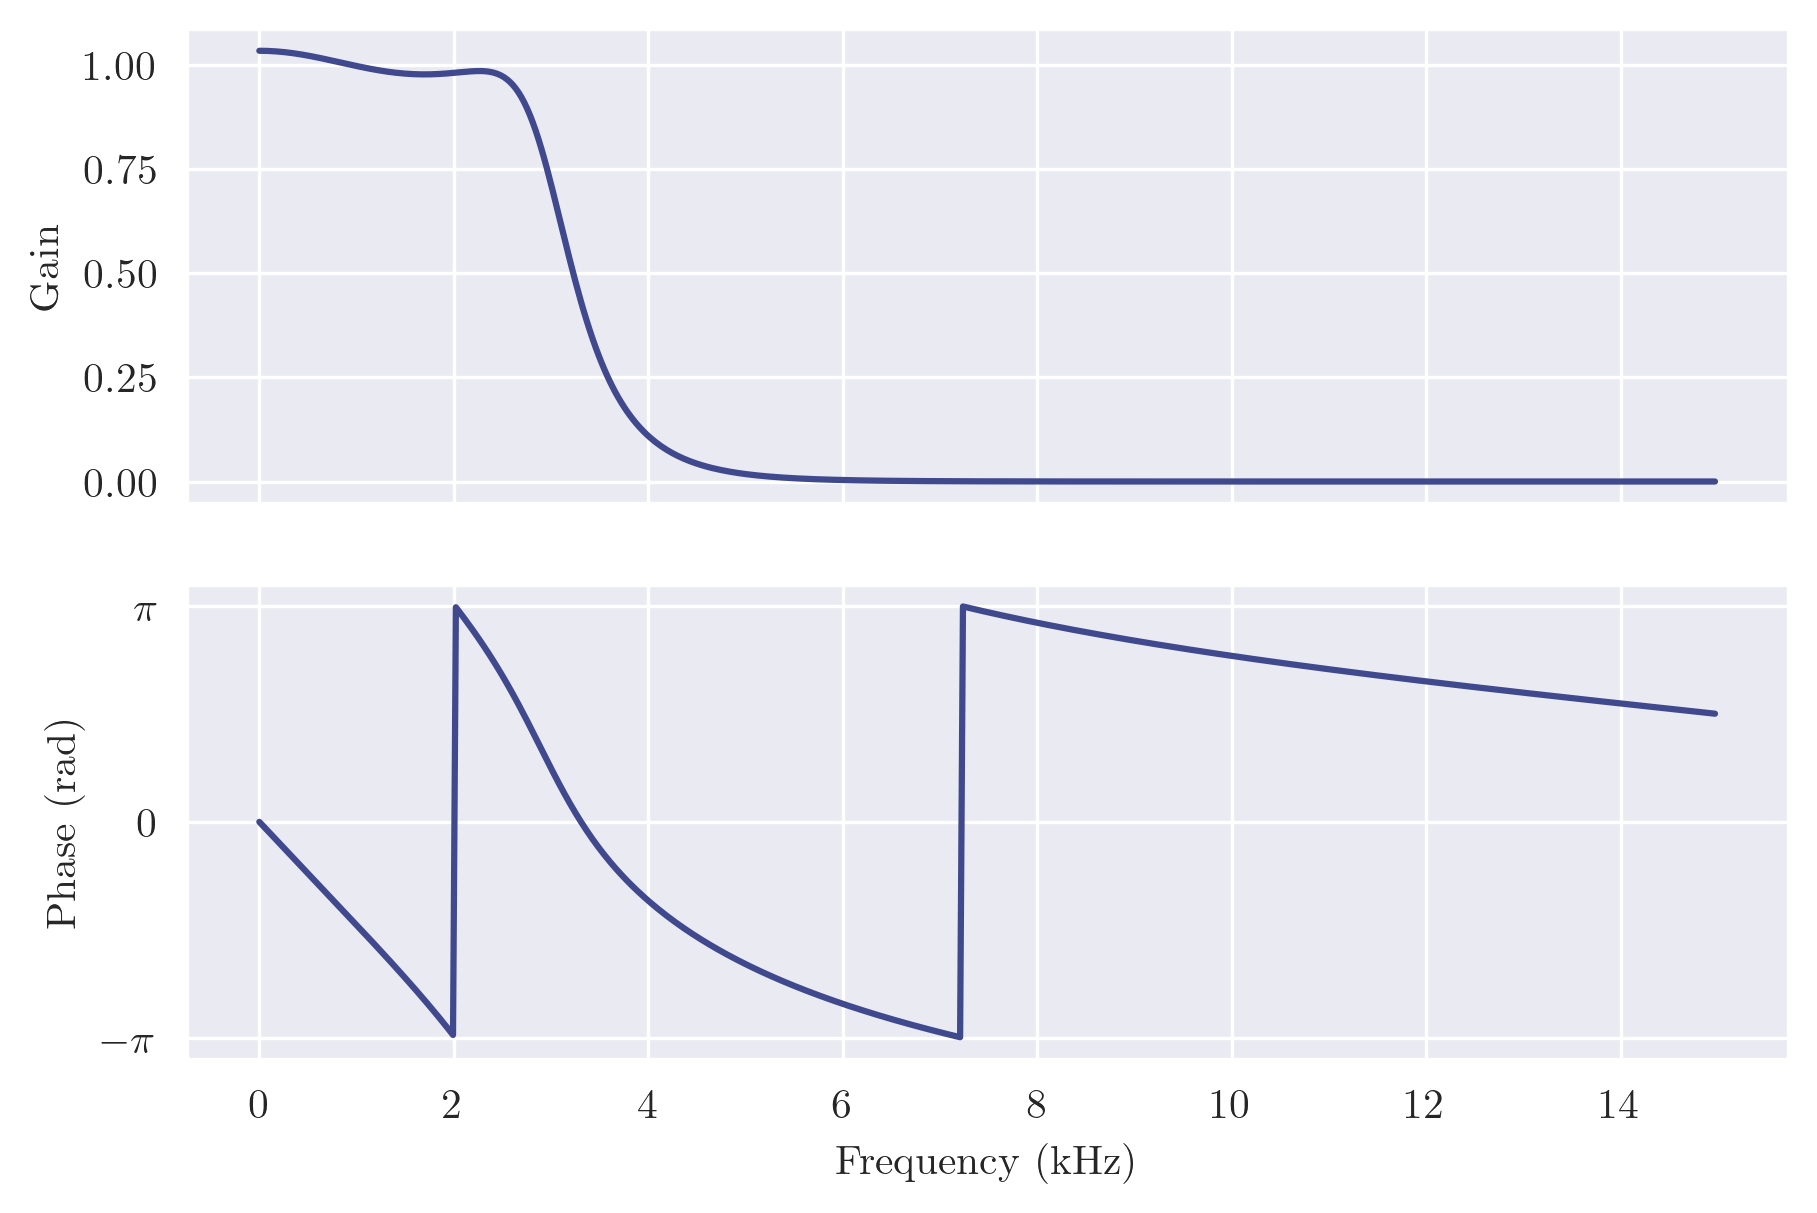
\includegraphics[width=\textwidth]{images/q8_q7th_freqz.png}
    \end{subfigure}
    \hfill
    \begin{subfigure}[b]{0.41\textwidth}
        \centering
        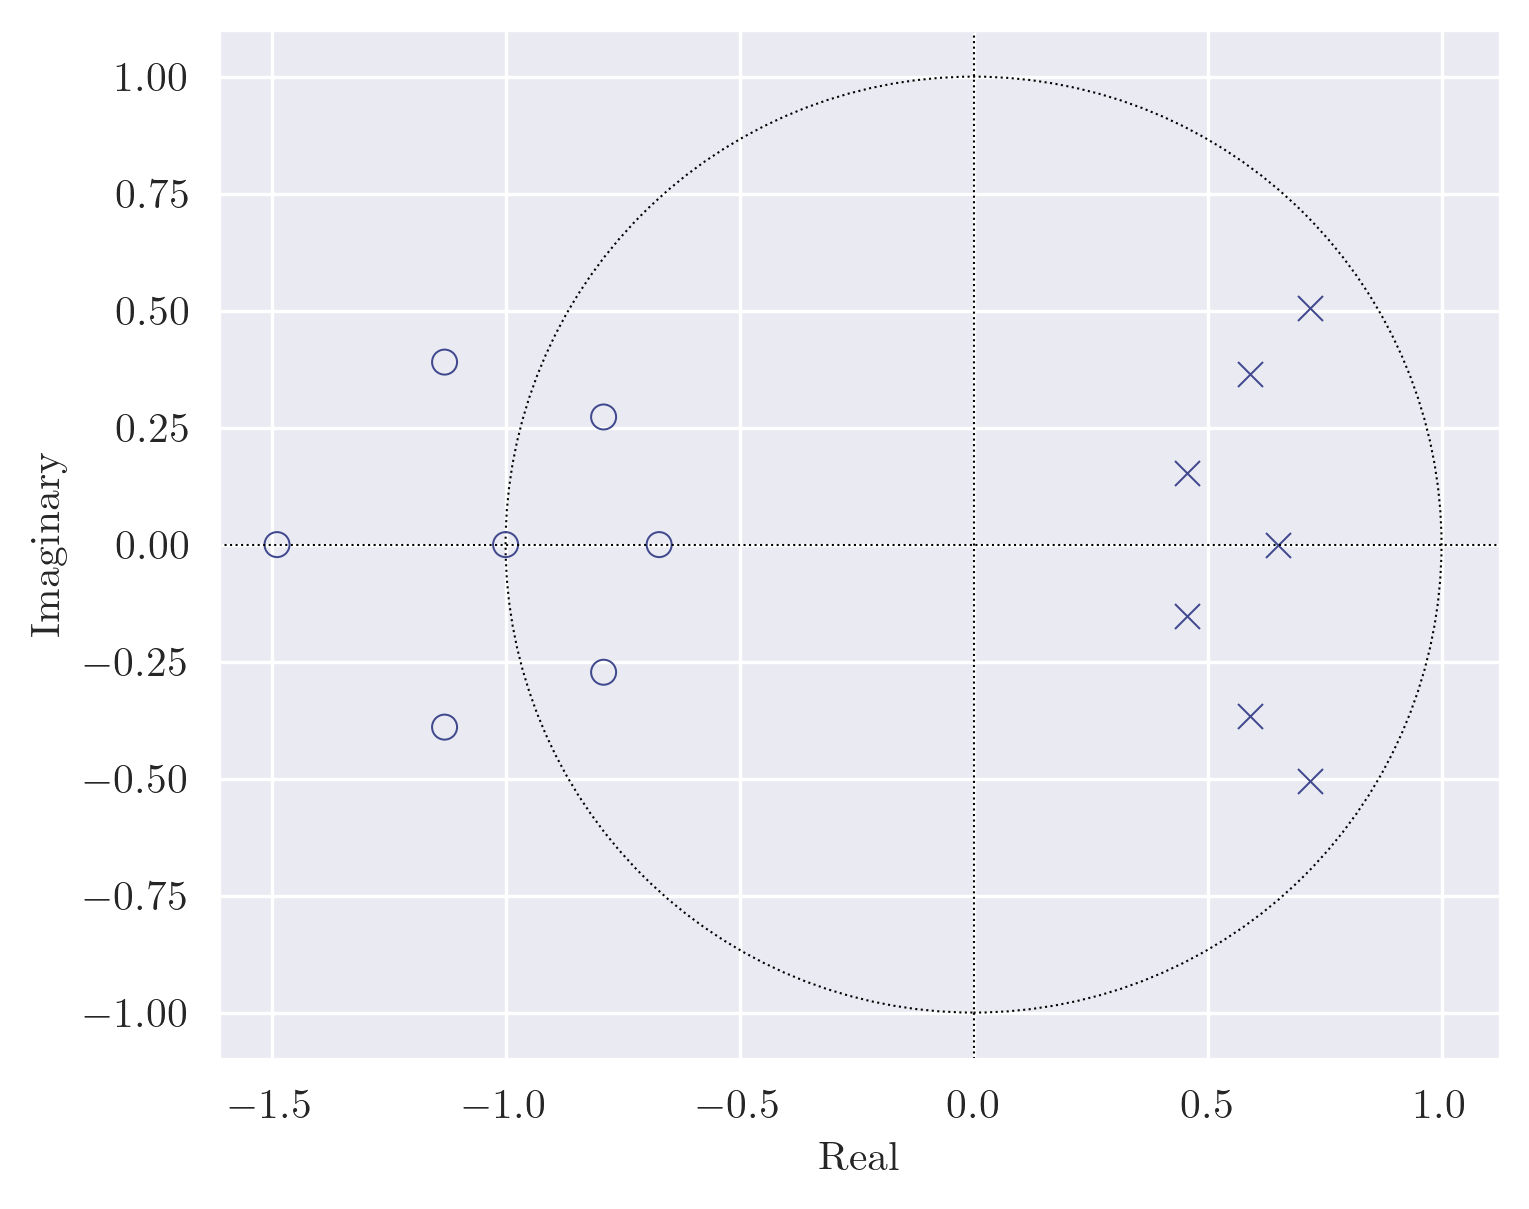
\includegraphics[width=\textwidth]{images/q8_q7th_zp.png}
    \end{subfigure}
    \caption{Frequency response and pole-zero plot of quantized 7th-order filter}
\end{figure}

\textit{TODO: describe observed differences}

\newpage

Finally, we attempt a 8th-order low pass Butterworth filter.

\begin{figure}[ht]
    \centering
    \begin{subfigure}[b]{0.58\textwidth}
        \centering
        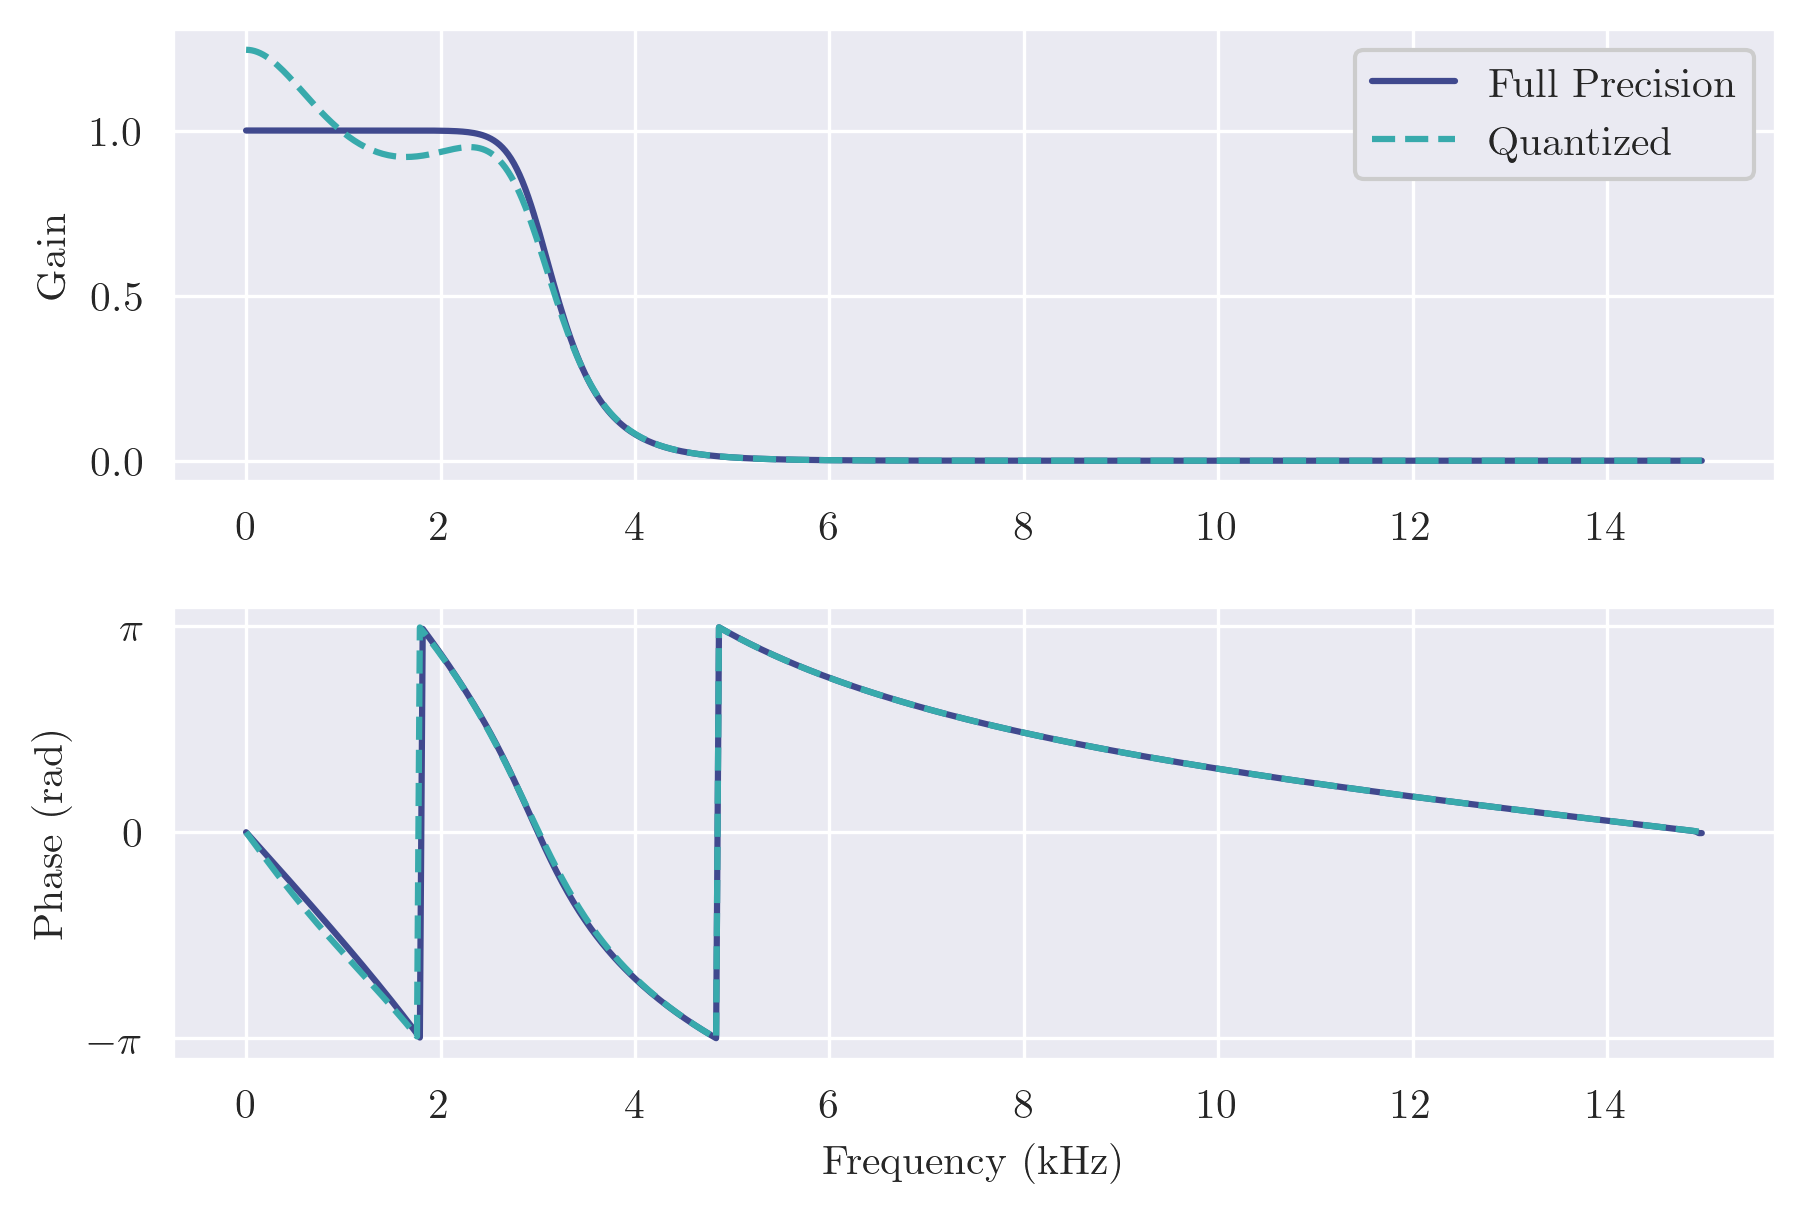
\includegraphics[width=\textwidth]{images/q8_8th_freqz.png}
    \end{subfigure}
    \hfill
    \begin{subfigure}[b]{0.41\textwidth}
        \centering
        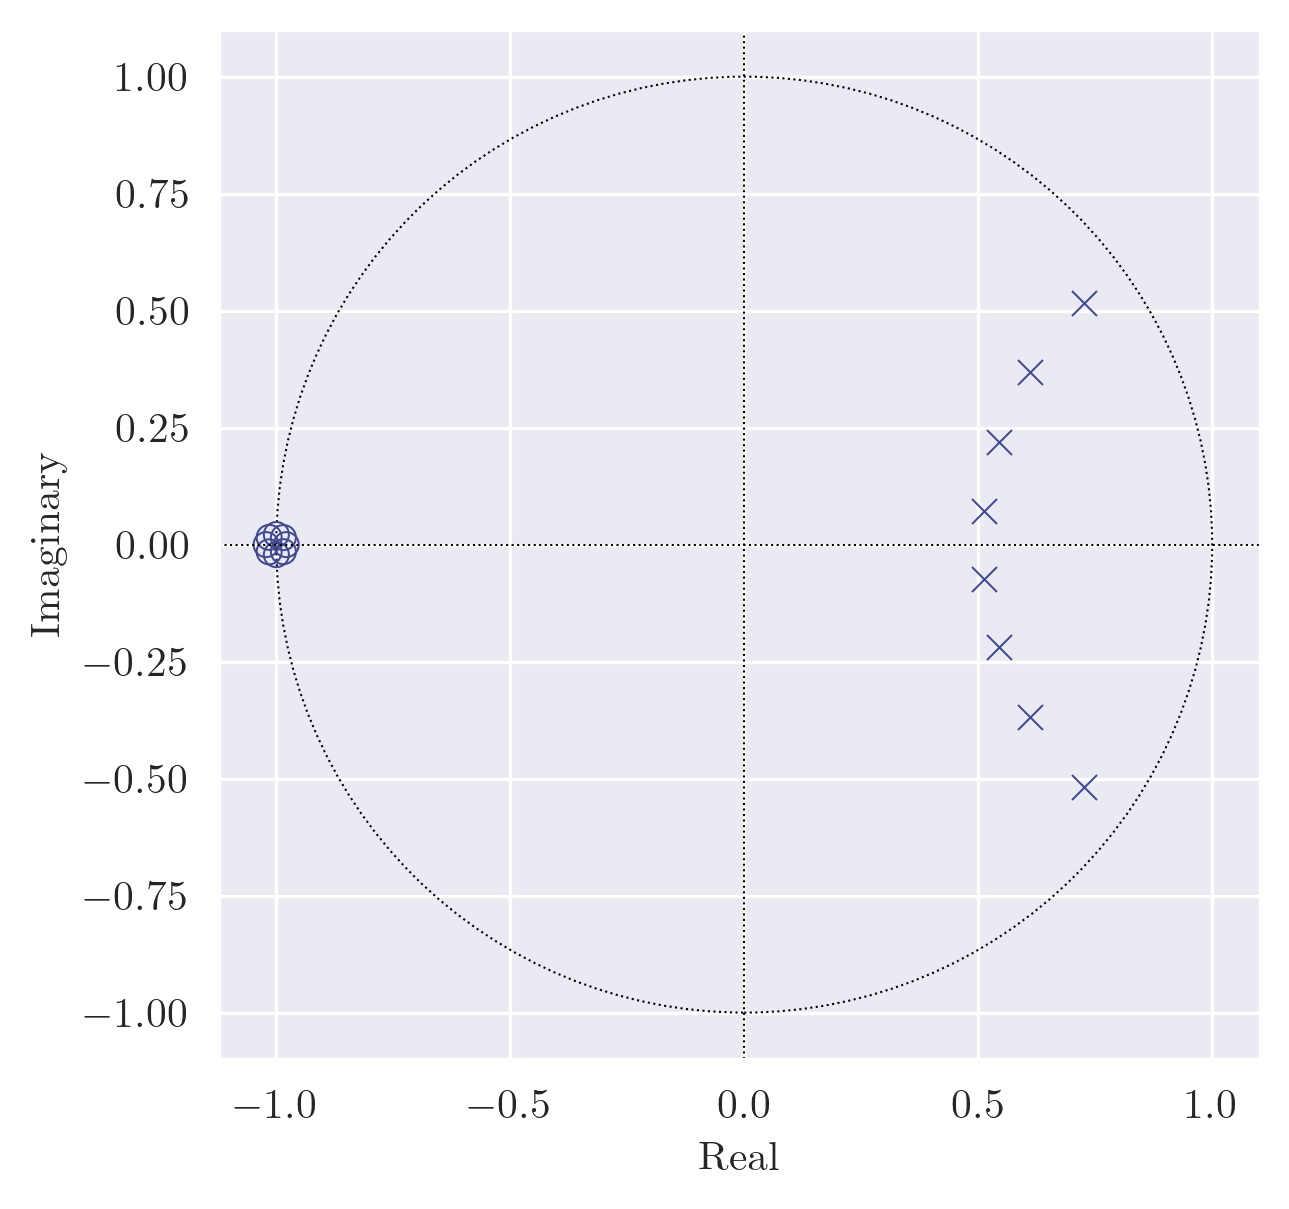
\includegraphics[width=\textwidth]{images/q8_8th_zp.png}
    \end{subfigure}
    \caption{Frequency response and pole-zero plot of 8th-order low pass Butterworth filter}
\end{figure}

We then quantize the filter coefficients and repeat, observing changes in the pole-zero plot.

\begin{figure}[!ht]
    \centering
    \begin{subfigure}[b]{0.58\textwidth}
        \centering
        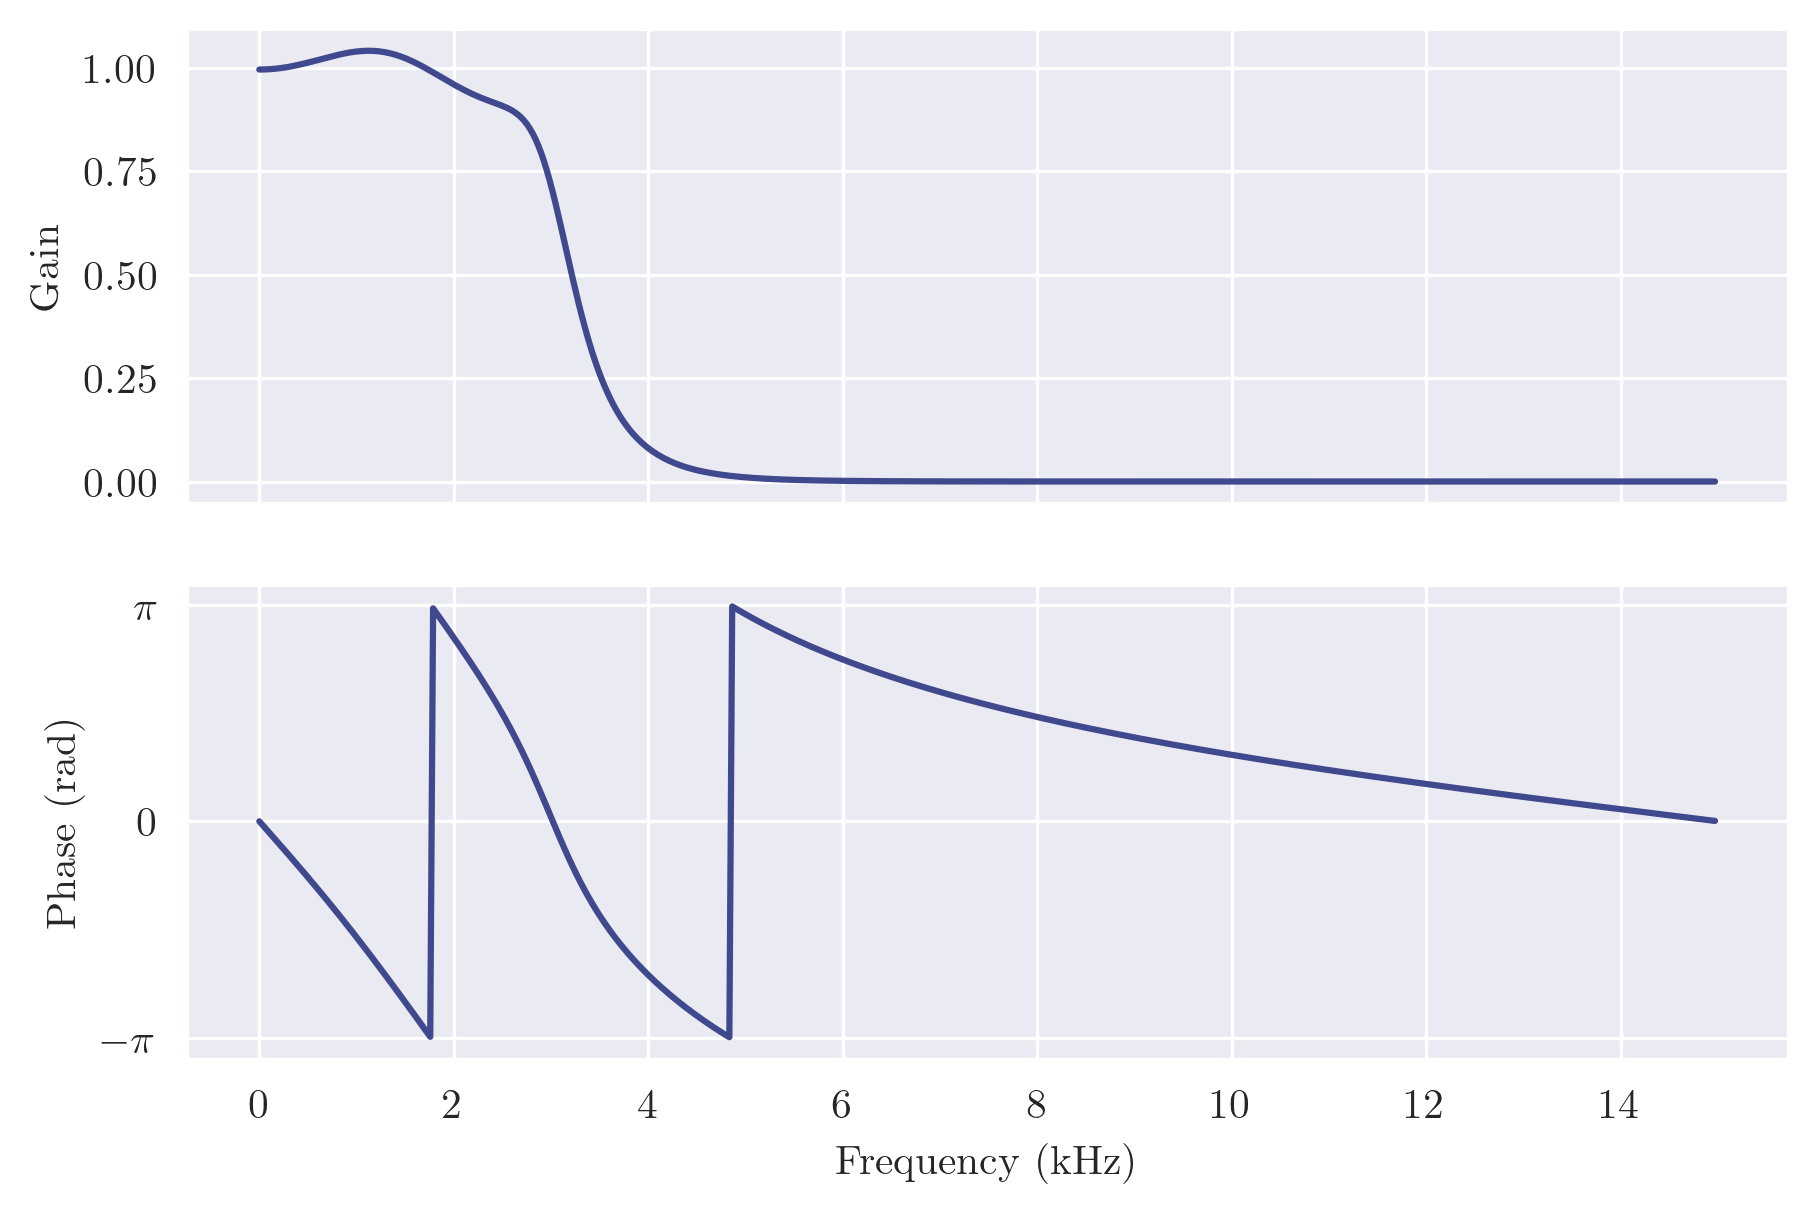
\includegraphics[width=\textwidth]{images/q8_q8th_freqz.png}
    \end{subfigure}
    \hfill
    \begin{subfigure}[b]{0.41\textwidth}
        \centering
        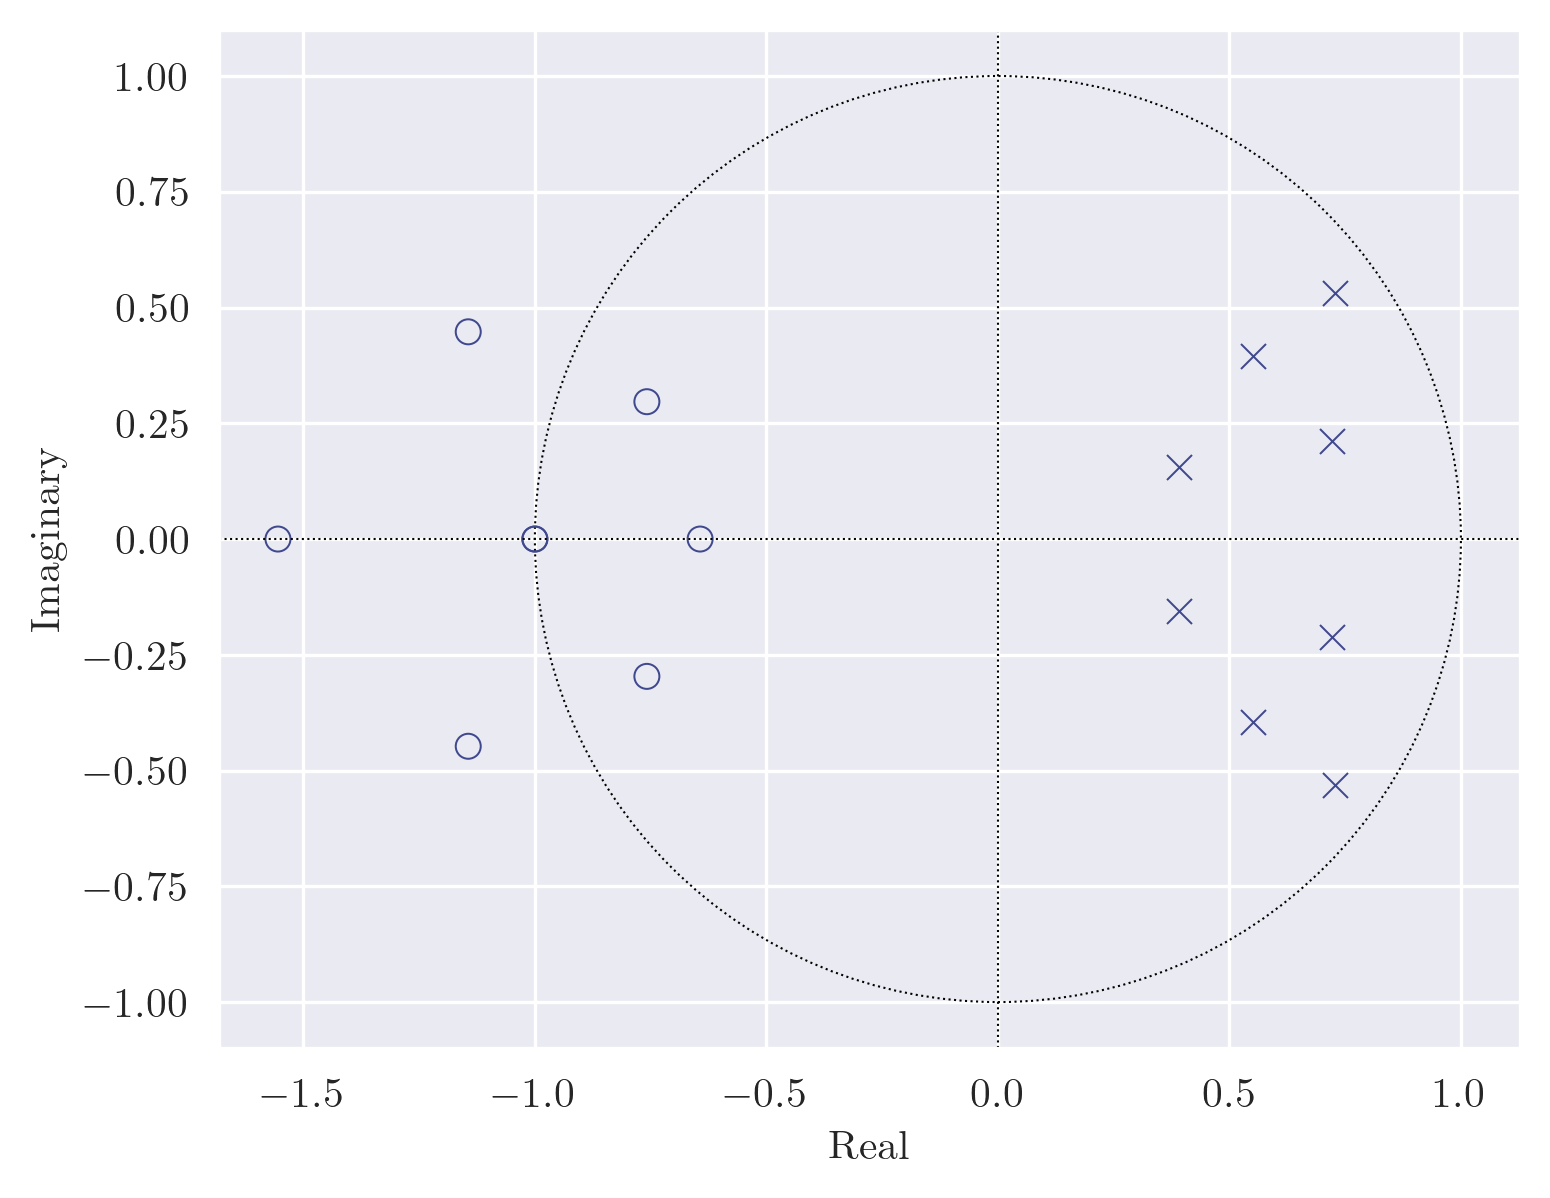
\includegraphics[width=\textwidth]{images/q8_q8th_zp.png}
    \end{subfigure}
    \caption{Frequency response and pole-zero plot of quantized 8th-order filter}
\end{figure}

\textit{TODO: describe observed differences}
